\section{Experiments}
\label{sec:Experiments}
characterizing the repeatability of one tag

%%%%%%%%%%%%%%%%%%%%
\subsection{Tag Characterization Experiments}

\begin{figure}[H]
	% Data

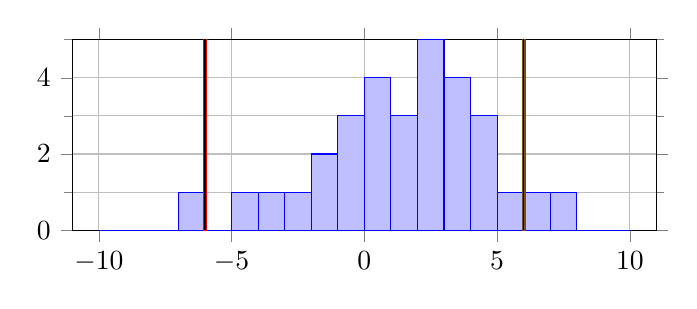
\begin{tikzpicture}
\begin{axis}[
height=4cm,
width=9cm,
%            ybar interval,      % <-- this causes the `xticks' to be centered
ymin= 0, ymax=5,
xmin=-11, xmax=11,
grid=both,
minor y tick num=1,
%yminorgrids=true,
tick align=outside, % <-- this positions the ticks "outside"
]
\addplot+ [
ybar interval,
mark=none,
fill=blue!25,   % fill the bars again
] coordinates {

	(-10,0)	%
	(-9,0)	%
	(-8,0)	%
	(-7,1)	%
	(-6,0)	%1
	(-5,1)	%11
	(-4,1)	%11
	(-3,1)	%111111
	(-2,2)	%11111
	(-1,3)	%111111
	 (0,4)	%11111
	 (1,3)	%1
	 (2,5)	%
	 (3,4)	%
	 (4,3)	%
	 (5,1)	%
	 (6,1)	%
	 (7,1)	%
	 (8,0)	%
	 (9,0)	%
	 (10,1)	%

};

\addplot+ [
ybar interval,
mark=none,
fill=black,   % fill the bars again
] coordinates {
	(-6.05,16) 
	(-5.95,16) 
};

\addplot+ [
ybar interval,
mark=none,
fill=black,   % fill the bars again
] coordinates {
	(6.05,16) 
	(5.95,16) 
};
\end{axis}

\end{tikzpicture}
	\caption{Histogram of one sensor face reading the same tag multiple times}
	\label{fig:histogram}
\end{figure}

We did some stuff, wrote it down here...

\begin{figure}[H]
	\begin{tikzpicture}
\begin{axis}[view={-20}{20}, grid=both]
\addplot3[surf] file {data.txt};
\end{axis}
\end{tikzpicture}
       
	\caption{Histogram of one sensor face reading the same tag multiple times}
	\label{fig:histogram}
\end{figure}

%%%%%%%%%%%%%%%%%%%%
\subsection{Crystalization Experiments}


We did some stuff, wrote it down here...
